\usetikzlibrary{patterns}

\begin{frame}{}
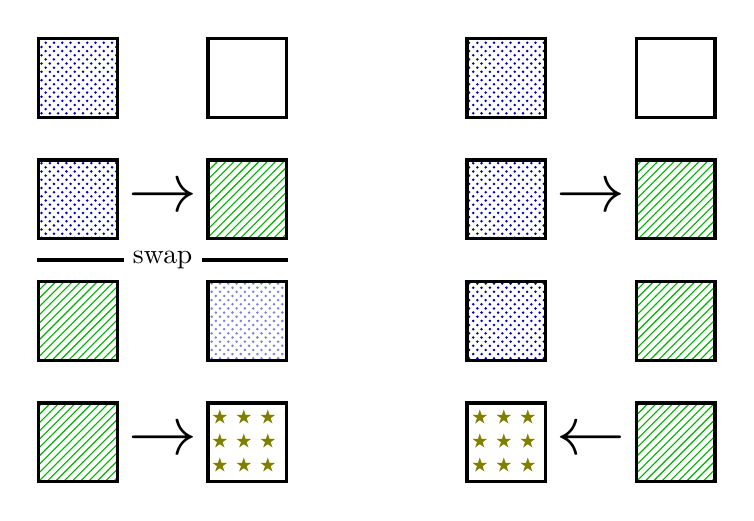
\begin{tikzpicture}
\tikzset{
    grid/.style={anchor=center,draw,very thick,minimum height=1cm,minimum width=1cm},
    grid A/.style={grid,pattern=crosshatch dots,pattern color=blue!70!black},
    grid B/.style={grid,pattern=north east lines,pattern color=green!70!black},
    grid C/.style={grid,pattern=fivepointed stars,pattern color=yellow!50!black},
    faded/.style={fill opacity=0.5},
    for arrow/.style={font=\Huge,anchor=center},
    ampersand replacement=\&,
}
\matrix[row sep=.5cm] (primary) {
    \node[grid A] {}; \& \node[for arrow] {~}; \& \node[grid] (first right) {}; \\
    \node[grid A] (first left) {}; \& \node[for arrow] {$\rightarrow$}; \& \node[grid B] (first right) {}; \\
    \node[grid B] {}; \& \node[for arrow] {~}; \& \node[grid A,faded] {}; \\
    \node[grid B] (second left) {}; \& \node[for arrow] {$\rightarrow$}; \& \node[grid C] (second right) {}; \\
};
    \draw[very thick] ([yshift=-2.5mm]first left.south west) -- ([yshift=-2.5mm]first right.south east)
        node[midway,fill=white]{swap};

\matrix[row sep=.5cm,anchor=north west] (secondary) at ([xshift=2cm]primary.north east) {
    \node[grid A] {}; \& \node[for arrow] {~}; \& \node[grid] {}; \\
    \node[grid A] {}; \& \node[for arrow] {$\rightarrow$}; \& \node[grid B] {}; \\
    \node[grid A] {}; \& \node[for arrow] {~}; \& \node[grid B] {}; \\
    \node[grid C] {}; \& \node[for arrow] {$\leftarrow$}; \& \node[grid B] {}; \\
};
\end{tikzpicture}
\end{frame}
